\documentclass[border=2pt]{standalone}
\usepackage{pgfplots}
\begin{document}
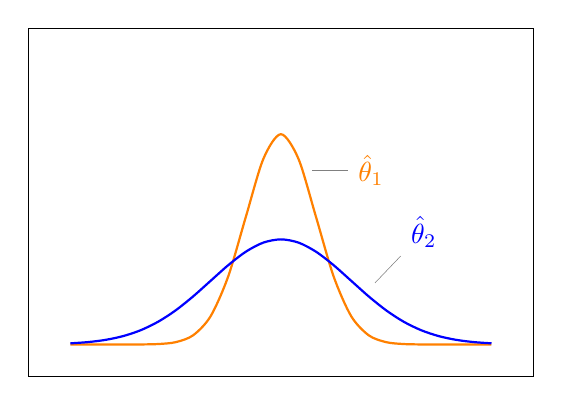
\begin{tikzpicture}[
  declare function={
    normalpdf(\x,\mu,\sigma)=(2*3.1415*\sigma^2)^(-0.5)*exp(-(\x-\mu)^2/(2*\sigma^2));
  }]
  \begin{axis}[width=8cm,height=6cm,ymax=0.6,domain=-6:6,samples=25,ticks=none]
    \addplot[smooth,thick,orange] {normalpdf(x,0,1)}
      node[pos=0.55,pin={right:$\hat{\theta}_1$}] {};
    \addplot[smooth,thick,blue] {normalpdf(x,0,2)}
      node[pos=0.7,pin={45:$\hat{\theta}_2$}] {};
  \end{axis}
\end{tikzpicture}
\end{document}
